\begin{name}
	{\tenchude}{ĐỀ ÔN TẬP SỐ 9}{LỚP TOÁN THẦY PHÁT}{\thoigian}
\end{name}
\setcounter{ex}{0}
\setcounter{bt}{0}
\Opensolutionfile{ans}[ans/ans-Vted-19-2023]
%%==========Câu 1
\begin{ex}%[Dự án 12-Vted-2022, Quan Ón]%[2D4Y1-2]
\immini{
 Điểm $M$ trong hình vẽ bên là điểm biểu diễn của số phức nào dưới đây?
 \choice
 {$z = -2 + 3i$}
 {\True $z = -3 + 2i$}
 {$z = 3 - 2i$}
 {$z = 2 - 3i$}
}{
 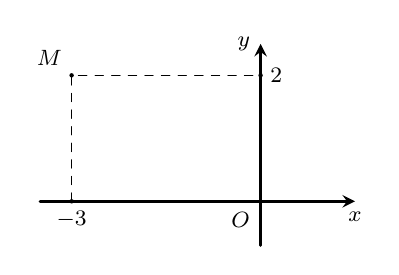
\begin{tikzpicture}[>=stealth,line join=round,line cap=round,font=\footnotesize,scale=0.8]
 	\draw[->,line width = 1pt] (-3.5,0)--(0,0) node[below left]{$O$}--(1.5,0) node[below]{$x$};
 	\draw[->,line width = 1pt] (0,-0.7) --(0,2.5) node[left]{$y$};
 	\fill (0,2) node[right]{$2$} circle (1pt);
 	\fill (-3,0) node[below]{$-3$} circle (1pt);
 	\draw [dashed] (-3,0)--(-3,2)--(0,2);
 	\fill (-3,2) node[above left]{$M$} circle (1pt);
 \end{tikzpicture}
}
\loigiai{
 Điểm $M$ trong hình vẽ bên là điểm biểu diễn của số phức $z = -3 + 2i$.
}
\end{ex}
%%==========Câu 2
\begin{ex}%[Dự án 12-Vted-2022, Quan Ón]%[2D1B5-1]
	Đường cong trong hình vẽ bên là đồ thị của hàm số nào sau đây?
	\begin{center}
	\begin{tikzpicture}[scale=0.7, font=\footnotesize, line join=round, line cap=round, >=stealth]
	\def\xt{-3.2} \def\xp{4.5} \def\yt{4} \def\yd{-2.5}
	\draw[->] (\xt,0)--(\xp,0) node [below]{$x$};
	\draw[->] (0,\yd)--(0,\yt) node [left]{$y$};
	\node at (0,0) [below left]{$O$} circle (1pt);
	\draw (1.09,0) node[below left]{$1$} circle (1pt);
	\draw (0,1) node[below right]{$1$} circle (1pt);
	\clip (\xt,\yd) rectangle (\xp,\yt);
	\draw [domain=-3.5:4.9, samples=100] %
	plot (\x, {((\x))/((\x) - 1)});
	\draw (-4,1)--(5,1);
	\end{tikzpicture}
	\end{center}
	\choice
	{$y = \dfrac{x+1}{x-1}$}
	{$y = \dfrac{x}{x+1}$}
	{\True $y = \dfrac{x}{x-1}$}
	{$y = \dfrac{x-2}{x+1}$}
\loigiai{
 Dựa vào đồ thị, ta thấy đồ thị hàm số có $x = 1$ là tiệm cận đứng, $y = 1$ là tiệm cận ngang và điểm $O(0;0)$ thuộc đồ thị. Do đó, đường cong trong hình vẽ là đồ thị của hàm số $y = \dfrac{x}{x-1}$.
}
\end{ex}
%%==========Câu 3
\begin{ex}%[Dự án 12-Vted-2022, Quan Ón]% [2D2Y4-1] 
Tập nghiệm của phương trình $3^{2x - 1} = 27$ là
\choice
{$\left\lbrace 1 \right\rbrace $}
{$\left\lbrace 5 \right\rbrace $}
{\True $\left\lbrace 2 \right\rbrace $}
{$\left\lbrace 4 \right\rbrace $}
\loigiai{
 Ta có
 $$ 3^{2x - 1} = 27 \Leftrightarrow 2x - 1 = \log_{3}27 \Leftrightarrow 2x - 1 = 3 \Leftrightarrow x = 2. $$
 Vậy tập nghiệm của phương trình $3^{2x - 1} = 27$ là $\left\lbrace 2 \right\rbrace $.
}
\end{ex}
%%==========Câu 4
\begin{ex}%[Dự án 12-Vted-2022, Quan Ón]% [2D2B4-1] 
Tập xác định của hàm số $y = \log_{3}(x+2)$ là
\choice
{$[-2;+\infty)$}
{\True $(-2;+\infty)$}
{$(2;+\infty)$}
{$[2;+\infty)$}
\loigiai{
 Điều kiện xác định $x + 2 > 0 \Leftrightarrow x > -2$.\\
 Vậy tập xác định của hàm số $y = \log_{3}(x+2)$ là $\mathcal{D} = (-2;+\infty)$.
}
\end{ex}
%%==========Câu 5
\begin{ex}%[Dự án 12-Vted-2022, Quan Ón]%[1D3B4-2] 
Cho cấp số nhân $(u_n)$ với $u_1 = 2$ và $u_4 = -16$. Công bội của cấp số nhân đã cho bằng
\choice
{$6$}
{$-6$}
{$-8$}
{\True $-2$}
\loigiai{
 Ta có $q^3 = \dfrac{u_4}{u_1} = \dfrac{-16}{2} = -8 \Rightarrow q = -2$.
}
\end{ex}
%%==========Câu 6
\begin{ex}%[Dự án 12-Vted-2022, Quan Ón]% [2H3Y1-1] 
Trong KG $Oxyz$, cho hai điểm $A(-1;3;5)$, $B(3;-5;1)$. Trung điểm của đoạn thẳng $AB$ có tọa độ là
\choice
{$(2;-2;6)$}
{$(2;-4;-2)$}
{\True $(1;-1;3)$}
{$(4;-8;-4)$}
\loigiai{
 Trung điểm của đoạn thẳng $AB$ có tọa độ là $(1;-1;3)$.
}
\end{ex}
%%==========Câu 7
\begin{ex}%[Dự án 12-Vted-2022, Quan Ón]%[2D3Y2-1] 
Cho $\displaystyle \int\limits_{0}^{1}f(x)dx = -4$, khi đó $\displaystyle -2\int\limits_{0}^{1}f(x)dx$ bằng
\choice
{$-2$}
{$2$}
{$-8$}
{\True $8$}
\loigiai{
 Vì $\displaystyle \int\limits_{0}^{1}f(x)dx = -4$ nên $\displaystyle -2\int\limits_{0}^{1}f(x)dx = -2\cdot (-4) = 8$.
}
\end{ex}
%%==========Câu 8
\begin{ex}%[Dự án 12-Vted-2022, Quan Ón]%[2D1Y2-2]
Cho hàm số $f(x)$ có bảng biến thiên như sau
\begin{center}
	
\begin{tikzpicture}[scale=1, font=\footnotesize, line join=round, line cap=round, >=stealth]
	\tkzTabInit[nocadre=false,lgt=1.2,espcl=2.5,deltacl=0.6]
	{$x$ /0.6,$f'(x)$ /0.6,$f(x)$ /1.6}
	{$-\infty$,$-2$,$-1$,$0$,$+\infty$}
	\tkzTabLine{,+,0,-,d,-,0,+,}
	\tkzTabVar{-/$-\infty$,+/$-3$,-D+/$-\infty$/$+\infty$,-/$1$,+/$+\infty$}
	\end{tikzpicture}
\end{center}
Giá trị cực tiểu của hàm số đã cho bằng
\choice
{$-2$}
{\True $1$}
{$0$}
{$-3$}
\loigiai{
 Dựa vào bảng biến thiên, giá trị cực tiểu của hàm số đã cho bằng $1$.
}
\end{ex}
%%==========Câu 9
\begin{ex}%[Dự án 12-Vted-2022, Quan Ón]%[2D3B2-1] 
Cho hàm số $f(x)$ liên tục trên $\mathbb{R}$ và $F(x)$ là một nguyên hàm của $f(x)$, biết $\displaystyle \int\limits_{0}^{9}f(x)dx = 9$ và $F(0)=3$. Khi đó giá trị $F(9)$ là
\choice
{$F(9) = -12$}
{\True $F(9) = 12$}
{$F(9) = -6$}
{$F(9) = 6$}
\loigiai{
 Ta có $\displaystyle \int\limits_{0}^{9}f(x)dx = 9 \Leftrightarrow F(9) - F(0) = 9 \Leftrightarrow F(9) - 3 = 9 \Rightarrow F(9) = 12$.
}
\end{ex}
%%==========Câu 10
\begin{ex}%[Dự án 12-Vted-2022, Quan Ón]% [2H3Y2-4] 
Trong KG $Oxyz$, mặt phẳng nào dưới đây đi qua điểm $M(1;-2;1)$?
\choice
{\True $(P_1)\colon x + y + z = 0$}
{$(P_2)\colon x + y + z - 1= 0$}
{$(P_3)\colon x - 2y + z = 0$}
{$(P_4)\colon x + 2y + z - 1= 0$}
\loigiai{
 Thay $x = 1$; $y = -2$; $z = 1$ vào phương trình của $(P_1)\colon x + y + z = 0$ ta được $1 + (-2) + 1 = 0 \Leftrightarrow 0 = 0$ (luôn đúng).\\
 Vậy mặt phẳng đi qua điểm $M(1;-2;1)$ là $(P_1)\colon x + y + z = 0$.
}
\end{ex}
%%==========Câu 11
\begin{ex}%[Dự án 12-Vted-2022, Thien Tran Xuan]%[2H3Y2-4]
Trong KG $Oxyz$, mặt phẳng nào dưới đây đi qua điểm $M(1; -2; 1)$?
\choice
{\True $(P_1) \colon x + y + z = 0$}
{$(P_2) \colon x + y + z - 1 = 0$}
{$(P_3) \colon x - 2y + z = 0$}
{$(P_4) \colon x + 2y + z - 1 = 0$}
\loigiai{
Do $1 - 2 + 1 = 0$ nên $M \in (P_1)$.
}
\end{ex}
%%==========Câu 12
\begin{ex}%[Dự án 12-Vted-2022, Thien Tran Xuan]%[2D4B1-1]
Môđun của số phức $z = 2 + 2i$ bằng
\choice
{$8$}
{\True $2\sqrt{2}$}
{$2$}
{$4$}
\loigiai{
Ta có $|z| = |2 + 2i| = \sqrt{2^2 + 2^2} =2\sqrt{2}$.
}
\end{ex}
%%==========Câu 13
\begin{ex}%[Dự án 12-Vted-2022, Thien Tran Xuan]%[2D4B2-2]
Cho hai số phức $z_1 = 2 + i$, $z_2 = -1 + 3i$. Số phức $z_1 + z_2$ có phần ảo bằng
\choice
{$4i$}
{$1$}
{$i$}
{\True $4$}
\loigiai{
Số phức $z_1 + z_2 = 1 + 4i$ có phần ảo bằng $4$.
}
\end{ex}
%%==========Câu 14
\begin{ex}%[Dự án 12-Vted-2022, Thien Tran Xuan]%[2D1Y2-2]
Cho hàm số $f(x)$ có bảng biến thiên của đạo hàm như sau:
\begin{center}
	
\begin{tikzpicture}
	\tkzTabInit[lgt=1.2,espcl=3]
	{$x$/1.2, $f(x)$/2.5}
	{$-\infty$,$-3$,$1$,$+\infty$}
	\tkzTabVar{+/$+\infty$,-/$-3$,+/$0$,-/$-\infty$}
	\end{tikzpicture}
\end{center}
Số điểm cực trị của hàm số đã cho là
\choice
{$3$}
{$0$}
{\True $2$}
{$1$}
\loigiai{
Số điểm cực trị của hàm số đã cho là $2$.
}
\end{ex}
%%==========Câu 15
\begin{ex}%[Dự án 12-Vted-2022, Thien Tran Xuan]%[2H3B1-3]
Trong KG $Oxyz$, mặt cầu có tâm là gốc toạ độ $O$ và đi qua điểm $M(0; 0; 2)$ có phương trình là
\choice
{$x^2 + y^2 + z^2 = 2$}
{\True $x^2 + y^2 + z^2 = 4$}
{$x^2 + y^2 + (z-2)^2 = 4$}
{$x^2 + y^2 + (z-2)^2 = 2$}
\loigiai{
Ta có $\vec{OM} = (0; 0; 2) \Rightarrow R = 2$.\\
Vậy mặt cầu có phương trình là $x^2 + y^2 + z^2 = 4$.
}
\end{ex}
%%==========Câu 16
\begin{ex}%[Dự án 12-Vted-2022, Thien Tran Xuan]%[1D2B2-1]
Có bao nhiêu cách xếp chỗ ngồi cho $3$ học sinh vào một dãy ghế dài gồm $5$ ghế trống, mỗi học sinh ngồi một ghế?
\choice
{$5!$}
{\True $\mathrm{A}_5^3$}
{$\mathrm{C}_5^3$}
{$5^3$}
\loigiai{
Số cách xếp chỗ ngồi cho $3$ học sinh vào một dãy ghế dài gồm $5$ ghế trống là $\mathrm{A}_5^3$.
}
\end{ex}
%%==========Câu 17
\begin{ex}%[Dự án 12-Vted-2022, Thien Tran Xuan]%[2H1Y3-2]
Một khối chóp có diện tích đáy bằng $6$ và chiều cao bằng $5$. Thể tích của khối chóp đó bằng
\choice
{\True $10$}
{$30$}
{$90$}
{$15$}
\loigiai{
Thể tích của khối chóp là $V = \dfrac{1}{3}Bh = 10$ (đvtt).
}
\end{ex}
%%==========Câu 18
\begin{ex}%[Dự án 12-Vted-2022, Thien Tran Xuan]%[2D1Y4-1]
Tiệm cận đứng của đồ thị hàm số $y = \dfrac{2x + 4}{x - 1}$ là đường thẳng
\choice
{\True $x = 1$}
{$x =-1$}
{$x = 2$}
{$x = -4$}
\loigiai{
Tiệm cận đứng của đồ thị hàm số $y = \dfrac{2x + 4}{x - 1}$ là đường thẳng $x = 1$.
}
\end{ex}
%%==========Câu 19
\begin{ex}%[Dự án 12-Vted-2022, Thien Tran Xuan]%[2D3Y1-1]
Họ nguyên hàm của hàm số $f(x) = x^{-5}$ là
\choice
{$-5x^{-6} + C$}
{$-4x^{-4} + C$}
{$\dfrac{1}{4}x^{-4} + C$}
{\True $-\dfrac{1}{4}x^{-4} + C$}
\loigiai{
Ta có $\displaystyle\int f(x) \mathrm{\,d}x = \displaystyle\int x^{-5} \mathrm{\,d}x = -\dfrac{1}{4}x^{-4} + C$.
}
\end{ex}
%%==========Câu 20
\begin{ex}%[Dự án 12-Vted-2022, Thien Tran Xuan]%[2H2B1-2]
Một hình nón có bán kính đáy $r = 3$ cm và độ dài đường sinh $l = 4$ cm. Diện tích xung quanh của hình nón đó bằng
\choice
{\True $12 \pi$cm $^2$}
{$48 \pi$cm $^2$}
{$24 \pi$cm $^2$}
{$36 \pi$cm $^2$}
\loigiai{
Diện tích xung quanh của hình nón là $S_{xq} = \pi r l = 12\pi$ cm$^2$.
}
\end{ex}
%----Thầy Đạt
\begin{ex}%[Dự án 12-Vted-2022, Tin Dat Tran]%[2D1Y5-4]
Đồ thị hàm số $y=\dfrac{x-4}{2 x+2}$ cắt trục hoành tại điểm có tung độ bằng
\choice
{$4$}
{$-2$}
{\True $0$}
{$-4$}
\loigiai{
Đồ thị hàm số $y=\dfrac{x-4}{2 x+2}$ cắt trục hoành tại điểm có tung độ bằng $0$.
}
\end{ex}
\begin{ex}%[Dự án 12-Vted-2022, Tin Dat Tran]%[2H3Y3-1]
Trong không gian $O x y z$, đường thẳng $d\colon \heva{&x=1-t \\ &y=2+2 t\\ &z=3+t}$ có một véc-tơ chỉ phương là
\choice
{\True $\overrightarrow{u_3}=(1 ;-2 ;-1)$}
{$\overrightarrow{u_4}=(1 ; 2 ; 3)$}
{$\overrightarrow{u_1}=(1 ; 2 ; 1)$}
{$\overrightarrow{u_2}=(1 ;-2 ; 1)$}
\loigiai{
Đường thẳng $d$ có một véc-tơ chỉ phương là $\overrightarrow{u}=\left(-1;2;1\right)\Rightarrow\overrightarrow{u_3}=-\overrightarrow{u}$ là véc-tơ chỉ phương của $d$.
}
\end{ex}
\begin{ex}%[Dự án 12-Vted-2022, Tin Dat Tran]%[2D2Y1-1]
Với $a$ là số thực dương tuỳ ý, $\sqrt{a^3}$ bằng
\choice
{$a^6$}
{\True $a^\frac{3}{2}$}
{$a^\frac{2}{3}$}
{$a^\frac{1}{6}$}
\loigiai{
Ta có $\sqrt{a^3}=a^\frac{3}{2}$.
}
\end{ex}
\begin{ex}%[Dự án 12-Vted-2022, Tin Dat Tran]%[2D2B5-2]
Tập nghiệm của bất phương trình $\log _2\left(x^2+5\right) \geq \log _2(2 x+8)$ là
\choice
{$[-1 ; 3]$}
{\True $(-4 ;-1] \cup[3 ;+\infty)$}
{$(-1 ; 3)$}
{$(-\infty ;-1] \cup[3 ;+\infty)$}
\loigiai{
Điều kiện: $\heva{&x^2+5>0\\&2x+8>0}\Leftrightarrow x>-4$.\\
	$\log _2\left(x^2+5\right) \geq \log _2(2 x+8)\Leftrightarrow x^2+5\geq 2x+8\Leftrightarrow x^2-2x-3\geq 0\Leftrightarrow\hoac{&x\leq -1\\&x\geq 3}$.
Kết hợp với điều kiện, ta được $\hoac{&-4<x\leq -1\\&x\geq 3}$.\\
Vậy tập nghiệm của bất phương trình là $(-4 ;-1] \cup[3 ;+\infty)$.
}
\end{ex}
\begin{ex}%[Dự án 12-Vted-2022, Tin Dat Tran]%[2H3B3-2]
Trong không gian $O x y z$, đường thẳng đi qua hai điểm $A(1 ; 2 ;-1)$ và $B(2 ;-1 ; 1)$ có PTTS là
\choice
{\True $\heva{&x=1+t \\ &y=2-3 t \\ &z=-1+2 t}$}
{$\heva{&x=1+t \\ &y=2-3 t \\ &z=1+2 t}$}
{$\heva{&x=1+t \\ &y=-3+2 t \\ &z=2-t}$}
{$\heva{&x=1+t \\ &y=1+2 t \\ &z=-t}$}
\loigiai{
Đường thẳng $AB$ có một véc-tơ chỉ phương là $\overrightarrow{AB}=\left(2-1;-1-2;1-(-1)\right)=\left(1;-3;2\right)$.\\
Suy ra PTTS của đường thẳng $AB$ là $\heva{&x=1+t \\ &y=2-3 t \\ &z=-1+2 t}$.
}
\end{ex}
\begin{ex}%[Dự án 12-Vted-2022, Tin Dat Tran]%[2H2Y2-1]
Một mặt cầu có bán kính bằng $2 r$ thì diện tích của nó bằng
\choice
{$4 \pi r^2$}
{$\dfrac{4}{3} \pi r^3$}
{$\dfrac{32}{3} \pi r^3$}
{\True $16 \pi r^2$}
\loigiai{
Diện tích của mặt cầu đã cho là $S=4\pi (2r)^2=16 \pi r^2$.
}
\end{ex}
\begin{ex}%[Dự án 12-Vted-2022, Tin Dat Tran]%[2D4B2-1]
Cho hai số phức $z_1=1+2 i$ và $z_2=2-5 i$, khi đó $z_1 \cdot \overline{z_2}$ bằng
\choice
{$-8-9 i$}
{$8-9 i$}
{$8+9 i$}
{\True $-8+9 i$}
\loigiai{
Ta có $\overline{z_2}=2+5i\Rightarrow z_1 \cdot \overline{z_2}=\left(1+2 i\right)\left(2+5i\right)=-8+9i$
}
\end{ex}
\begin{ex}%[Dự án 12-Vted-2022, Tin Dat Tran]%[2D2B4-2]
Đạo hàm của hàm số $y=5^{2 x}$ là
\choice
{\True$y'=5^{2 x} \ln 25$}
{$y'=\dfrac{5^{2 x}}{\ln 5}$}
{$y'=5^{2 x} \ln 5$}
{$y'=\dfrac{5^{2 x}}{\ln 25}$}
\loigiai{
$y=5^{2 x}\Rightarrow y'=5^{2x}\cdot \ln5\cdot (2x)'=5^{2x}\cdot 2\ln5=5^{2x}\ln5^2=5^{2x}\ln25$.
}
\end{ex}
\begin{ex}%[Dự án 12-Vted-2022, Tin Dat Tran]%[2D1B3-1]
Giá trị lớn nhất của hàm số $f(x)=x^4-2 x^2+3$ trên đoạn $[0 ; 2]$ bằng
\choice
{\True $11$}
{$12$}
{$10$}
{$13$}
\loigiai{
Ta có $y'=4x^3-4x$.\\
$y'=0\Leftrightarrow \hoac{&x=0\in\left[0;2\right]\\&x=1\in\left[0;2\right]\\&x=-1\notin\left[0;2\right]}$.\\
$f(0)=3$; $f(1)=2$; $f(2)=11$.
Vậy giá trị lớn nhất của hàm số $f(x)=x^4-2 x^2+3$ trên đoạn $[0 ; 2]$ bằng $11$.
}
\end{ex}
\begin{ex}%[Dự án 12-Vted-2022, Tin Dat Tran]%[1D2B5-4]
Chọn ngẫu nhiên hai số trong 15 số nguyên dương đầu tiên. Xác suất để hai số được chọn có tổng là một số lẻ bằng
\choice
{\True $\dfrac{8}{15}$}
{$\dfrac{11}{15}$}
{$\dfrac{4}{15}$}
{$\dfrac{1}{7}$}
\loigiai{
Tập hợp gồm 15 số nguyên dương đầu tiên là $\left\{1;2;3;\cdots;15\right\}$.\\
Số cách chọn 2 số nguyên trong 15 số nguyên dương đầu tiên là $\mathrm{C}^{2}_{15}$ cách.\\
Để tổng hai số được chọn có tổng là một số lẻ thì trong hai số đó phải có 1 số chẵn và một số lẻ:
\begin{itemize}
	\item Chọn 1 số chẵn thuộc $A$ có $7$ cách.
	\item Chọn 1 số lẻ thuộc $A$ có $8$ cách.
\end{itemize}
Chọn 2 số thuộc $A$ để tổng hai số được chọn có tổng là một số lẻ có $7\cdot 8=56$ cách.\\
Xác suất cần tìm là $\dfrac{56}{\mathrm{C}^{2}_{15}}=\dfrac{8}{15}$.
}
\end{ex}
%---Cô Hồng
%%==========Câu 31
\begin{ex}%[Dự án 12-Vted-2022, Cô Hồng]%[2D2Y3-2]
Biết rằng $\log _2 3=a, \log _2 5=b$. Tính $\log _{45} 4$ theo $a$ và $b$ ta được kết quả nào dưới đây?
\choice
{ $\dfrac{2 b+a}{2}$}
{ $2 a b$}
{$\True\dfrac{2}{2 a+b}$}
{$\dfrac{2 a+b}{2}$}
\loigiai{Ta có $\log _{45} 4=\dfrac{1}{\log _{4} 45}=\dfrac{2}{\log _{2} (5\cdot 9)}=\dfrac{2}{\log _{2} 5+2\log _{2} 3}=\dfrac{2}{2a+b}\cdot$
}
\end{ex}
%%==========Câu 32
\begin{ex}%[Dự án 12-Vted-2022, Cô Hồng]%[2H3B2-3]
Trong không gian $O x y z$, cho ba điểm $A(3 ;-1 ; 2)$, $B(4 ;-1 ;-1)$, $C(2 ; 0 ; 2)$. Mặt phẳng đi qua ba điểm $A, B, C$ có phương trình
\choice
{$3 x-3 y+z-14=0$}
{$3 x-2 y+z-8=0$}
{\True $3 x+3 y+z-8=0$}
{$2 x+3 y-z+8=0$}
\loigiai{ Ta có $ \overrightarrow{AB}=(1;0;-3), \overrightarrow{AC}=(-1;1;0) $.\\
Gọi	$\overrightarrow{n}=[\overrightarrow{AB},\overrightarrow{AC}]=(3;3;1)$.\\
Khi đó mặt phẳng đi qua ba điểm $A, B, C$ là mặt phẳng đi qua điểm $A$ và nhận $\overrightarrow{n}$ làm véc-tơ pháp tuyến.
Suy ra $(ABC)$ có phương trình $\colon$ \begin{center}
	$3\cdot (x-3)+3\cdot(y+1)+1\cdot(z-2)=0\Leftrightarrow 3x+3y+z-8=0$.
\end{center}
}
\end{ex}
%%==========Câu 33
\begin{ex}%[Dự án 12-Vted-2022, Cô Hồng]%[2D3K3-1]
Diện tích hình phẳng $(H)$ được gạch chéo trong hình vẽ được giới hạn bởi đồ thị của hai hàm số $y=f(x), y=x^2+4 x$ và hai đường thẳng $x=-2 ; x=0$.
Biết $\displaystyle \int\limits_{-2}^0 f(x) \mathrm{\,d} x=\dfrac{4}{3}$, diện tích hình phẳng $(H)$ là
\choice
{$\dfrac{7}{3}$}
{$\dfrac{16}{3}$}
{ $\dfrac{4}{3}$}
{\True $\dfrac{20}{3}$}
\begin{center}
	\begin{tikzpicture}[>=stealth,line join=round,line cap=round,font=\footnotesize,scale=1,x=.7cm,y=.8cm,declare function={
	f(\x)=(\x)^2+4*(\x);
	g(\x)=2-(\x)^2;
	}]
	\draw[->] (0,-5)--(0,3)node[right]{$y$};
	\draw[->] (-5,0)--(3,0)node[below]{$x$};
	\fill[pattern=north east lines,pattern color=red] plot[domain=-2:0]
	(\x,{f(\x)})--plot[domain=0:-2](\x,{g(\x)});
	\draw[thick,samples=150,smooth,domain=-4.6:.6] plot(\x,{f(\x)});
	\draw[thick,samples=150,smooth,domain=-2.6:2] plot(\x,{g(\x)});
	\draw[dashed] (-2,0)--(-2,-4);
	\fill (-2,0)circle(1pt)node[above]{$-2$}
	(0,0)circle(1pt)node[below right]{$O$}
	(-2,-2)circle(1pt)
	(-2,-4)circle(1pt)
	;
	\path
	(2,{g(2)})node[below]{$y=f(x)$}
	(.6,{f(.5)})node[above right]{$y=x^2+4x$};
\end{tikzpicture}
\end{center}
\loigiai{Diện tích hình $(\mathrm{H})$ là 
	$$
	\begin{aligned}
	& S=\int\limits_{-2}^0\left[f(x)-\left(x^2+4 x\right)\right] \mathrm{\,d} x \\
	& =\int\limits_{-2}^0 f(x) \mathrm{\,d} x-\int\limits_{-2}^0\left(x^2+4 x\right) \mathrm{\,d} x \\
	& =\dfrac{4}{3}-\left.\left(\frac{x^3}{3}+2 x^2\right)\right|_{-2} ^0 \\
	& =\dfrac{4}{3}+\dfrac{(-2)^3}{3}+2(-2)^2=\dfrac{20}{3}
	\end{aligned}
	$$
	Vậy diện tích hình (H) là $S=\dfrac{20}{3}$.
}
\end{ex}
%%==========Câu 34
\begin{ex}%[Dự án 12-Vted-2022, Cô Hồng]%[2H1B3-2]
Cho khối lăng trụ $A B C.A' B' C'$ có thể tích bằng $a^3$. Gọi $M$ là trung điểm cạnh $A A'$. Thể tích của khối chóp $M . A B C$ bằng
\choice
{$\dfrac{a^3}{3}$}
{$\dfrac{a^3}{4}$}
{$\dfrac{a^3}{2}$}
{\True $\dfrac{a^3}{6}$}
\loigiai{ \immini{Gọi $h, h'$ lần lượt là đường cao hạ từ đỉnh $A$ và $M$ xuống mặt phẳng $(A' B' C')$.\\ Vì $M$ là trung điểm của $AA'$ suy ra $h'=\dfrac{h}{2}$.\\
	Khi đó $V_{M.ABC}=\dfrac{1}{3}S_{\triangle ABC}\cdot h'= \dfrac{1}{3}S_{\triangle ABC}\cdot\dfrac{h}{2}=\dfrac{1}{6}V_{ABC.A' B' C'}=\dfrac{a^3}{6}\cdot$}
{\begin{tikzpicture}
	\def\a{4}
	\def\h{4.5}
	\path (0:0) coordinate (A)
	++(0:\a) coordinate (B)
	++(-150:\a/2) coordinate (C)
	($(A)+(80:\h)$) coordinate (A')
	($(A')+(B)-(A)$) coordinate (B')
	($(B')+(C)-(B)$) coordinate (C');
	\coordinate[label=left:$M$] (M) at ($(A)!0.5!(A')$);
	\draw[dashed] (A)--(B)--(M);
	\draw (C)--(C') 	(B)--(B') 	(A)--(A')
	(A)--(C)--(B) (A')--(B')--(C')--cycle (A)--(C)--(M);
	\foreach \x/\g in {A/180,B/-45,C/0,A'/180,B'/-45,C'/0}
	\fill[black] 	(\x) circle (1pt)
	($(\g:4mm)+(\x)$) node {$\x$};
	\end{tikzpicture}
}}
\end{ex}
%%==========Câu 35
\begin{ex}%[Dự án 12-Vted-2022, Cô Hồng]%[2D3B2-3]
Xét $u=\ln (x+1)$ và $v=x^2$, khi đó $\displaystyle\int\limits_0^1 u \mathrm{\,d}v$ bằng
\choice
{$x^2 \ln (x+1)\bigg|_0 ^1-\displaystyle\int\limits_0^1 2 x \ln (x+1) \mathrm{\,d}x$}
{\True $x^2 \ln (x+1)\bigg|_0 ^1- \displaystyle\int\limits_0^1 \frac{x^2}{x+1} \mathrm{\,d}x$}
{$x^2 \ln (x+1)\bigg|_0 ^1+\displaystyle\int\limits_0^1 2 x \ln (x+1) \mathrm{\,d}x$}
{$x^2 \ln (x+1)\bigg|_0 ^1+\displaystyle\int\limits_0^1 \frac{x^2}{x+1} \mathrm{\,d}x$}
\loigiai{
Ta có $\mathrm{\,d} u=\dfrac{ \mathrm{\,d}x}{x+1}$ suy ra \\
$\displaystyle\int\limits_0^1 u\mathrm{\,d} v= uv\bigg|_0 ^1-\displaystyle\int\limits_0^1 v \mathrm{\,d}u=x^2 \ln (x+1)\bigg|_0 ^1- \displaystyle\int\limits_0^1 \dfrac{x^2}{x+1} \mathrm{\,d}x $.
}
\end{ex}
%%==========Câu 36
\begin{ex}%[Dự án 12-Vted-2022, Cô Hồng]%[2H1K3-4]
\immini{Cho hình chóp đều $S . A B C D$ có độ dài cạnh đáy bằng 2 và độ dài cạnh bên bằng $2 \sqrt{2}$ (tham khảo hình bên). Góc giữa đường thẳng $S C$ và mặt phẳng $(A B C D)$ bằng
\choice
{$30^{\circ}$}
{$45^{\circ}$}
{\True $60^{\circ}$}
{$90^{\circ}$}}
{
	\begin{tikzpicture}[line join=round,line cap=round, font=\footnotesize,scale=1,>=stealth]
	\def\r{1.8}
	\path
	(0,0) coordinate (O)
	(-\r,0) coordinate (m)
	(\r,0) coordinate (N)
	(10:1.5*\r) coordinate (B)
	(90:2*\r) coordinate (S)
	($(m)+(B)-(N)$) coordinate (A)
	($(B)!2!(O)$) coordinate (D)
	($(A)!2!(O)$) coordinate (C)
	;
	\draw (S)--(B)-- (C) --(D)--(S)(S)--(C);
	\draw[dashed] (S)--(A)--(B)(A)--(D);
	\foreach \x/\g in {S/90,A/180,B/0,C/-80,D/180}\fill[black] (\x) circle(1pt)+(\g:0.3)node{$\x$};
	\end{tikzpicture}}
\loigiai{\immini{ Gọi $O$ là giao điểm của $AC$ và $BD$.\\
	Vì $S . A B C D$ là hình chóp đều nên $SO\perp (ABCD)$ suy ra góc giữa đường thẳng $S C$ và mặt phẳng $(A B C D)$ bằng $(SC,OC)=\widehat{SCO} $.\\
	Trong tam giác vuông $SOC$ ta có $\cos\widehat{OCS} =\dfrac{OC}{SC}=\dfrac{\sqrt{2}}{2\sqrt{2}}=\dfrac{1}{2}\cdot$\\
	Suy ra $\widehat{SCO}=60^\circ$.\\
	Vậy góc giữa đường thẳng $S C$ và mặt phẳng $(A B C D)$ bằng $60^{\circ}$.}
{
	\begin{tikzpicture}[line join=round,line cap=round, font=\footnotesize,scale=1,>=stealth]
	\def\r{1.8}
	\path
	(0,0) coordinate (O)
	(-\r,0) coordinate (m)
	(\r,0) coordinate (N)
	(10:1.5*\r) coordinate (B)
	(90:2*\r) coordinate (S)
	($(m)+(B)-(N)$) coordinate (A)
	($(B)!2!(O)$) coordinate (D)
	($(A)!2!(O)$) coordinate (C)
	;
	\draw (S)--(B)-- (C) --(D)--(S)(S)--(C);
	\draw[dashed] (S)--(A)--(B)(A)--(D)(A)--(C)(S)--(O)(B)--(D);
	\foreach \x/\g in {S/90,A/180,B/0,C/-80,D/180,O/-90}\fill[black] (\x) circle(1pt)+(\g:0.3)node{$\x$};
\end{tikzpicture}}
}
\end{ex}
%%==========Câu 37
\begin{ex}%[Dự án 12-Vted-2022, Cô Hồng]%[2H1K3-4]
 \immini{Cho hình hộp chữ nhật $A B C D. A' B' C' D'$ có $A B=A D=2$ và $A A'=2 \sqrt{2}$ (tham khảo hình bên).
 Khoảng cách giữa hai đường thẳng $A' C$ và $A B$ bằng
\choice
{$\sqrt{2}$}
{2}
{\True $\dfrac{2 \sqrt{6}}{3}$}
{$\dfrac{2 \sqrt{10}}{5}$}}
{	\begin{tikzpicture}[line cap=round,line join=round,font=\footnotesize,>=stealth,scale=1.1]
	\fill (0,0) coordinate [label=left:$B$] (A) circle(1pt)
	(4,0) coordinate (B) node[shift={(-90:1ex)}]{$C$} circle(1pt)
	(40:2) coordinate [label=left:$A$] (D) circle(1pt)
	(90:3) coordinate [label=left:$B'$] (A') circle(1pt)
	($(B)+(D)$) coordinate [label=right:$D$] (C) circle(1pt)
	($(A')+(B)$) coordinate [label=above:$C'$] (B') circle(1pt)
	($(A')+(C)$) coordinate [label=right:$D'$] (C') circle(1pt)
	($(A')+(D)$) coordinate [label=above:$A'$] (D') circle(1pt);
	\draw (C')--(B')--(A')--(A) (C)--(C')--(D')--(A') (B')--(B) (A)--(B)--(C) ;
	\draw [dashed] (A)--(D)--(D') (D)--(C) (D')--(B) ;
	\end{tikzpicture}
}
\loigiai{
\immini{
Ta có $AB\parallel CD$ suy ra $\mathrm{d}(AB,A'C )=\mathrm{d}[AB,(A'CD)]=\mathrm{d}[A,(A'CD)]$.\\
Mà $ S_{\triangle ACD}=\dfrac{1}{2}AD\cdot CD=2 $ nên $ V_{A'ACD}=\dfrac{1}{3}A'A\cdot S_{\triangle ACD}=\dfrac{4\sqrt{2}}{3}\cdot $\\
Ta lại có: $A'C=\sqrt{AC^2+AA'^2}=2;A'D=\sqrt{AD^2+AA'^2}=2\sqrt{3}$.\\
Suy ra $S_{\triangle A'CD}=\sqrt{(3+\sqrt{3})(\sqrt{3}+1)(3-\sqrt{3})(\sqrt{3}-1)}=\sqrt{12}$.\\
Khi đó $\mathrm{d}[A,(A'CD)]=\dfrac{3V_{A'ACD}}{S_{\triangle A'CD}}=\dfrac{2 \sqrt{6}}{3}\cdot$\\
Vậy khoảng cách giữa hai đường thẳng $A' C$ và $A B$ bằng $\dfrac{2 \sqrt{6}}{3}\cdot$
}{	\begin{tikzpicture}[line cap=round,line join=round,font=\footnotesize,>=stealth,scale=1.1]
	\fill (0,0) coordinate [label=left:$B$] (A) circle(1pt)
	(4,0) coordinate (B) node[shift={(-90:1ex)}]{$C$} circle(1pt)
	(40:2) coordinate [label=left:$A$] (D) circle(1pt)
	(90:3) coordinate [label=left:$B'$] (A') circle(1pt)
	($(B)+(D)$) coordinate [label=right:$D$] (C) circle(1pt)
	($(A')+(B)$) coordinate [label=above:$C'$] (B') circle(1pt)
	($(A')+(C)$) coordinate [label=right:$D'$] (C') circle(1pt)
	($(A')+(D)$) coordinate [label=above:$A'$] (D') circle(1pt);
	\draw (C')--(B')--(A')--(A) (C)--(C')--(D')--(A') (B')--(B) (A)--(B)--(C) ;
	\draw [dashed] (A)--(D)--(D') (B)--(D)--(C) (C)-- (D')--(B) ;
\end{tikzpicture}
}}
\end{ex}
%%==========Câu 38
\begin{ex}%[Dự án 12-Vted-2022, Trương Đăng Khoa]%[2D1G5-3]
	Cho hàm số $f(x)$ có bảng biến thiên như sau:
	\begin{center}
	
\begin{tikzpicture}[scale=1, font=\footnotesize]
	\tkzTabInit[nocadre=false, lgt=1.2, espcl=2, deltacl=0.6]
	{$x$/0.8,$f'(x)$/0.6,$f(x)$/2}
	{$-\infty$,$-1$,$2$,$+\infty$};
	\tkzTabLine{,+,$0$,-,$0$,+,};
	\tkzTabVar{-/$-\infty$,+/$5$,-/$-3$,+/$+\infty$};
	\end{tikzpicture}
	\end{center}
	Số nghiệm thực phân biệt của phương trình $f'\left[f(x)+2\right]=0$ là
	\choice
	{$6$}
	{$5$\True}
	{$4$}
	{$3$}
	\loigiai{
	$f'\left[f(x)+2\right]=0\Leftrightarrow \hoac{& f(x)+2=-1 \\ &f(x)+2=2}\Leftrightarrow \hoac{ &f(x)=-3\\ &f(x)=0.}$\\
	Ta có
	\begin{itemize}
	\item $f(x)=-3$ $\Rightarrow$ phương trình có $2$ nghiệm.
	\item $f(x)=0$ $\Rightarrow$ phương trình có $3$ nghiệm.
	\end{itemize}
	Vậy $f'\left[f(x)+2\right]=0$ có $5$ nghiệm.
	}
\end{ex}
%%==========Câu 39
\begin{ex}%[Dự án 12-Vted-2022, Trương Đăng Khoa]%[2D2G6-4]
	Có bao nhiêu giá trị nguyên $m$, ($m\geq 2$) sao cho có không quá $4$ số nguyên $x$ thỏa mãn $m^{-x}\cdot 3^{x^2}<1$?
	\choice
	{$241$}
	{$79$}
	{$242$\True}
	{$80$}
	\loigiai{
	Xét $\begin{aligned}[t]
	&m^{-x}\cdot 3^{x^2}<1\\
	\Leftrightarrow&\dfrac{1}{m^2}\cdot (3^x)^x<1\\
	\Leftrightarrow & 3^x)^x<m^2.
	\end{aligned}$\\
	Trường hợp $1$. $x>0$, khi đó
	$\begin{aligned}[t]
	&3^x<m\\
	\Leftrightarrow& x<\log_3 m\\
	\Rightarrow & x\in (0;\log_3 m).
	\end{aligned}$\\
	Theo yêu cầu bài toán $\Rightarrow 0<\log_3 m \leq 5$.\\
	$\Rightarrow 1<m\leq 243$.\\
	Mà $m\geq 2$, $m$ nguyên do đó $m\in\{2;3;\ldots;243\}$.\\
	Trường hợp $2$. $x<0$, khi đó $\begin{aligned}[t]
	&3^x>m\\
	\Leftrightarrow& x>\log_3 m\\
	\Rightarrow &x\in (\log_3 m;0).
	\end{aligned}$\\
	Yêu cầu bài toán $\Rightarrow -5\leq \log_3 m<0$.\\
	$\Rightarrow \dfrac{1}{242}\leq m<1$ (loại).
	}
\end{ex}
%%==========Câu 40
\begin{ex}%[Dự án 12-Vted-2022, Trương Đăng Khoa]%[2D3G1-3]
	Cho hàm số $f(x)$ có đạo hàm $f'(x)=\ln (x+1)$, $\forall x\in (-1;+\infty)$. Khi $\displaystyle\int\limits_{0}^{1} f(x)\mathrm{\,d}x=0$ thì $f(0)$ bằng.
	\choice
	{$-\dfrac{5}{4}+2\ln 2$}
	{$\dfrac{3}{4}-2\ln 2$}
	{$\dfrac{5}{4}-2\ln 2$\True}
	{$-\dfrac{3}{4}+2\ln 2$}
	\loigiai{
	\begin{itemize}
	\item Ta có $f'(x)=\ln (x+1)$ $\Rightarrow f(x)=\displaystyle\int \ln (x+1)\mathrm{\,d}x$.\\
	Đặt $\heva{ &u=\ln (x+1)\Rightarrow \mathrm{\,d}u=\dfrac{1}{x+1}\\
	&dv=dx\Rightarrow v=x.}$\\
	$\begin{aligned}[t]
	\Rightarrow f(x)&=x\cdot \ln(x+1)-\displaystyle\int \dfrac{x}{x+1}\mathrm{\,d}x\\
	&=x\cdot\ln (x+1)-\displaystyle\int \left(x-\dfrac{1}{x+1}\right)\mathrm{\,d}x\\
	&=x\cdot \ln (x+1)-x+\ln (x+1)+\mathrm{C}\\
	&=(x+1)\cdot\ln (x+1)-x+\mathrm{C}.
	\end{aligned}$\\
	\item Đặt $F(x)=\displaystyle\int\limits_{0}^{1} f(x)\mathrm{\,d}x=F(1)-F(0)$.\\
	\item Xét $\begin{aligned}[t]
	\displaystyle\int f(x)\mathrm{\,d}x&=\displaystyle\int \left[(x+1)\cdot\ln (x+1)-x+\mathrm{C}\right]\\
	&=\displaystyle\int(x+1)\cdot \ln (x+1)\mathrm{\,d}x-\dfrac{x^2}{2}+\mathrm{C}x.
	\end{aligned}$\\
	\item Đặt $I=\displaystyle\int(x+1)\cdot \ln (x+1)\mathrm{\,d}x$.\\
	Đặt $\heva{&u=\ln (x+1)\Rightarrow \mathrm{\,d}u=\dfrac{1}{x+1}\\ &dv=(x+1)\mathrm{\,d}x=\Rightarrow v=\dfrac{x^2}{2}+x.}$\\
	$\begin{aligned}[t]
	I&=\left(\dfrac{x^2}{2}+x\right)\cdot \ln (x+1)-\dfrac{1}{2}\displaystyle\int \dfrac{x^2+2x}{x+1}\mathrm{\,d}x\\
	&=\left(\dfrac{x^2}{2}+x\right)\cdot \ln (x+1)-\dfrac{1}{2} \displaystyle\int\left[ (x+1)-\dfrac{1}{x+1}\right] \mathrm{\,d}x\\
	&=\left(\dfrac{x^2}{2}+x\right)\cdot \ln (x+1)-\dfrac{1}{2}\left[\dfrac{x^2}{2}+x-\ln (x+1)\right]\\
	&=\left(\dfrac{x^2}{2}+x+\dfrac{1}{2}\right)\cdot \ln (x+1)-\dfrac{x^2}{4}-\dfrac{x}{2}.
	\end{aligned}$\\
	\item Khi đó $F(x)=\left(\dfrac{x^2}{2}+x+\dfrac{1}{2}\right)\cdot \ln (x+1)-\dfrac{3}{4}x^2-\dfrac{x}{2}+\mathrm{C}x$.
	\item $F(1)=2\cdot \ln 2-\dfrac{5}{4}+\mathrm{C}$.
	\item $F(0)=0$.
	\item Ta có $F(x)=0\Leftrightarrow F(1)-F(0)=0\Rightarrow \mathrm{C}=\dfrac{5}{4}-2\cdot\ln 2$.\\
	$\Rightarrow f(x)=(x+1)\cdot\ln (x+1)-x+\dfrac{5}{4}-2\cdot\ln 2$.\\
	$\Rightarrow f(0)=\dfrac{5}{4}-2\ln 2$.
	\end{itemize}
	}
\end{ex}
%%==========Câu 41
\begin{ex}%[Dự án 12-Vted-2022, Trương Đăng Khoa]%[2H3K1-1]
	Trong KG $Oxyz$, cho đường thẳng $d\colon \dfrac{x-1}{2}=\dfrac{y-2}{-2}=\dfrac{z+1}{1}$ và mặt phẳng $(P)\colon x+y+z-2=0$. Xét điểm $M$ thuộc $(P)$ và điểm $N$ thuộc $d$ sao cho $\vv{OM}=-2\vv{ON}$, khi đó $MN$ bằng.
	\choice
	{$\sqrt{21}$}
	{$3\sqrt{105}$\True}
	{$\sqrt{105}$}
	{$3\sqrt{21}$}
	\loigiai{
	Goi $N(2t+1;-2t+2;t-1)\in d\Rightarrow\overrightarrow{OM}=-2\overrightarrow{ON}=(-4t-2;4t-4;-2t+2)$.\\
	Mặt khác $M\in(P)\Leftrightarrow(-4t-2)+(4t-4)+(-2t+2)-2=0\Leftrightarrow t=-3$.\\
	$\Rightarrow M(10;-16;8)$, $N(-5;8;-4)\Rightarrow MN=3\sqrt{105}$.
	}
\end{ex}
%%==========Câu 42
\begin{ex}%[Dự án 12-Vted-2022, Trương Đăng Khoa]%[2H1G3-4]
	Cho khối lăng trụ đều $ABC.A'B'C'$ có độ dài cạnh đáy bằng $2a$. Côsin góc giữa hai mặt phẳng $(ABC')$ và $(BCC'B')$ bằng $\dfrac{1}{2\sqrt{3}}$. Thể tích khối lăng trụ đã cho bằng. 
	\choice
	{$\dfrac{3a^3\sqrt{2}}{4}$}
	{$\dfrac{a^3\sqrt{2}}{2}$}
	{$\dfrac{3a^3\sqrt{2}}{2}$\True}
	{$\dfrac{3a^3\sqrt{2}}{8}$}
	\loigiai{
	\begin{center}
	\begin{tikzpicture}
	\path
	(0,0) coordinate (B)
	(4,0) coordinate (A)
	(2.5,1) coordinate (C)
	(0,5) coordinate (B')
	(4,5) coordinate (A')
	(2.5,6) coordinate (C')
	($(B)!0.5!(C)$) coordinate (M)
	($(B)!0.25!(C')$) coordinate (H)
	($(B)!0.6!(C')$) coordinate (K)
	;
	\path pic[draw,angle radius=7pt,fill=teal] {right angle=M--H--B};
	\path pic[draw,angle radius=7pt,fill=teal] {right angle=C--K--B};
	\path pic[draw,angle radius=7mm] {angle=M--H--A};
	\draw (B)--(A)--(A')--(C')--(B')--(B) (A')--(B');
	\draw[dashed] (A)--(C')--(B) (A)--(C)--(B) (C)--(C') (A)--(M) (M)--(H) (C)--(K) (A)--(H);
	\foreach \x/\g in{A/-90,B/-90,A'/90, C'/90, B'/90, C/40, M/-90, H/140, K/140}
	\fill[black] (\x) circle (1.2pt) ($(\x)+(\g:3mm)$) node {$\x$};
	\end{tikzpicture}
	\end{center}
	Với $AB=BC=CA=2a$, đặt $CC'=x$, $(x>0)$.\\
	Gọi $M$ là trung điểm $BC$ và kẻ $MH\perp BC'\Rightarrow BC'\perp(AMH)\Rightarrow\left((ABC'),(BCC'B')\right)=\widehat{AHM}$.\\
	Ta có $\cos\widehat{AHM}=\dfrac{1}{2\sqrt{3}}\Rightarrow\tan\widehat{AHM}=\sqrt{\dfrac{1}{\cos^2\widehat{AHM}}-1}=\sqrt{11}\Rightarrow\cot\widehat{AHM}=\dfrac{1}{\sqrt{11}}$.\\
	Vậy $MH=AM\cdot\widehat{AHM}=\dfrac{\sqrt{3}}{2}\cdot 2a\cdot\dfrac{1}{\sqrt{11}}=\sqrt{\dfrac{3}{11}}a$.\\
	Kẻ $CK\perp BC'\Rightarrow MH\parallel CK\Rightarrow MH=\dfrac{1}{2} CK=\dfrac{CB\cdot CC'}{2\sqrt{CB^2+CC^{' 2}}}=\dfrac{x}{\sqrt{x^2+4}}$.\\
	Suy ra $\dfrac{x}{\sqrt{x^2+4}}=\sqrt{\dfrac{3}{11}}a\Leftrightarrow x=\dfrac{\sqrt{6}}{2}a\Rightarrow V_{ABC.A'B'C'}=S_{ABC}\cdot CC'=\dfrac{\sqrt{3}}{4}\cdot (2a)^2\cdot\dfrac{\sqrt{6}}{2}a=\dfrac{3\sqrt{2}}{2}a^3$.
	}
\end{ex}
%%==========Câu 43
\begin{ex}%[Dự án 12-Vted-2022, Trương Đăng Khoa]%[2D1G1-3]
	Cho hàm số $f(x)$ có đạo hàm $f'(x)=x^2-x-2$, $\forall x\in\mathbb{R}$. Số giá trị nguyên của tham số $m\in [-20;20]$ để hàm số $g(x)=f(2x^3-3x^2-12x+m)$ nghịch biến trên khoảng $(-1;2)$ là
	\choice
	{$19$}
	{$18$}
	{$16$}
	{$13$\True}
	\loigiai{
	Ta có $\begin{aligned}[t]
	g(x)&=f(2x^3-3x^2-12x+m)\\
	g'(x)&=\left(6x^2-6x-12\right)\cdot f'\left(2x^3-3x^2-12x+m\right).
	\end{aligned}$\\
	Hàm số $g(x)$ nghịch biến trên khoảng $(-1;2)$ $\Leftrightarrow g'(x)\leq 0$, $\forall x\in(-1;2)$.\\
	Ta xét $6x^2-6x-12\leq 0$, $\forall x\in(-1;2)$.\\
	$\Rightarrow f'\left(2x^3-3x^2-12x+m\right)\geq 0$, $\forall x\in(-1;2)$\quad $(1)$.\\
	Mặt khác $f'(x)\geq 0\Leftrightarrow x^2-x-2\geq 0\Leftrightarrow \hoac{&x\geq 2\\ &x\leq -1.}$\\
	Do đó $(1)\Leftrightarrow \hoac{ &2x^3-3x^2-12x+m\geq 2\\
	&2x^3-3x^2-12x+m\leq -1}$, $\forall x\in(-1;2)$\quad $(2)$.\\
	Đặt hàm số $u(x)=2x^3-3x^2-12x+m$ có bảng biến thiên trên đoạn $[-1;2]$ như sau
	\begin{center}
	
\begin{tikzpicture}[scale=1, font=\footnotesize]
	\tkzTabInit[nocadre=false, lgt=1.2, espcl=2, deltacl=0.6]
	{$x$/0.8,$u'(x)$/0.6,$u(x)$/2}
	{$-1$,$2$};
	\tkzTabLine{,-,};
	\tkzTabVar{+/$m+7$,-/$m-20$};
	\end{tikzpicture}
	\end{center}
	Vậy $(2)\Leftrightarrow \hoac{&m-20\geq 2\\ &m+7\leq -1}\Leftrightarrow\hoac{&m\geq 22\\ &m\leq -8}\Rightarrow m\in\{-20;\ldots;-8\}$.
	}
\end{ex}
%%==========Câu 44
\begin{ex}%[Dự án 12-Vted-2022, Trương Đăng Khoa]%[2D4G4-1]
	Trên tập số phức, xét phương trình $z^2+a z+b=0,(a,b\in\mathbb{R})$. Có bao nhiêu cặp $(a;b)$ để phương trình đã cho có hai nghiệm phức là $z_1,z_2$ thoả mãn $(2z_1+z_2)\overline{z}_1=5+2\sqrt{2} i$?
	\choice 
	{$2$}
	{$3$}
	{$4$\True}
	{$1$}
	\loigiai{
	\begin{itemize}
	\item Cách $1$.\\
	Xét $\Delta=a^2-4b$.\\
	Trường hợp $1$. Nếu $\Delta\ge 0\Rightarrow z_1$, $z_2\in\mathbb{R}\Rightarrow(2z_1+z_2)\overline{z}_1\in\mathbb{R}\ne 5+2\sqrt{2} i$ (loại)\\
	Trường hợp $2$. Nếu $\Delta<0\Rightarrow z_{1,2}=\dfrac{-a\pm\sqrt{4b-a^2}\cdot i}{2}$.\\
	Khi đó $\begin{aligned}[t]
	(2z_1+z_2)\overline{z}_1&=2z_1\overline{z}_1+z_2\overline{z}_1\\&=2|z_1|^2+z_2^2\\&=2b+\dfrac{1}{4}\left[a^2-\left(4b-a^2\right)\pm 2a\sqrt{4b-a^2}\cdot i\right]\\
	&=b+\dfrac{1}{2} a^2\pm\dfrac{1}{2} a\sqrt{4b-a^2}\cdot i\\&=5+2\sqrt{2} i\Leftrightarrow \heva{
	&b+\dfrac{1}{2}a^2=5\quad (1)\\
	&a\sqrt{4b-a^2}=\pm 4\sqrt{2}\quad (2).
	}
	\end{aligned}$\\
	Từ $(1)$ $\Rightarrow a^2=10-2b;(2)\Rightarrow a^2\left(4b-a^2\right)=32$.\\
	$\Rightarrow(10-2b)(4b-10+2b)=32\Leftrightarrow-12b^2+80b-132=0\Leftrightarrow \hoac{& b=3\Rightarrow a^2=4\\ & b=\dfrac{11}{3}\Rightarrow a^2=\dfrac{8}{3}}\Rightarrow (a;b)=(\pm 2;3)$; $\left(\pm\sqrt{\dfrac{8}{3}};\dfrac{11}{3}\right)$.
	\item Cách $2$. Xét tương tự Cách 1, ở Trường hợp $2$ đặt $z_1=x+y i$, ($x$, $y\in\mathbb{R}$) $\Rightarrow z_2=\overline{z}_1=x-y i$ khi đó\\
	$\begin{aligned}[t]
	&(2z_1+z_2)\overline{z_1}=5+2\sqrt{2} i\Leftrightarrow[2(x+y i)+(x-y i)](x-y i)=5+2\sqrt{2} i\\
	\Leftrightarrow& (3x+y i)(x-y i)=5+2\sqrt{2} i\Leftrightarrow 3x^2+y^2-2x y=5+2\sqrt{2} i\Leftrightarrow \heva{ & 3x^2+y^2=5\quad (1)\\ &-2xy=2\sqrt{2} \quad (2).}
	\end{aligned}$ \\
	Từ $(2)\Rightarrow y=-\dfrac{\sqrt{2}}{x}$ thay vào $(1)$ $\Rightarrow 3x^2+\dfrac{2}{x^2}=5\Leftrightarrow 3x^4-5x^2+2=0\Leftrightarrow \hoac{ & x^2=1 \\ &x^2=\dfrac{2}{3}}\Rightarrow (x;y)=\left(-1;\sqrt{2}\right)$; $\left(1;-\sqrt{2}\right)$; $\left(-\sqrt{\dfrac{2}{3}};\sqrt{3}\right)$; $\left(\sqrt{\dfrac{2}{3}};-\sqrt{3}\right)$.\\
	Với mỗi cặp $(x;y)$ theo vi-ét có $\heva{ &a=-(z_1+z_2)=-2x\\ & b=z_1z_2=x^2+y^2}$ $\Rightarrow$ có $1$ cặp $(a;b)$ tương ứng.\\
	Vậy có $4$ cặp $(a;b)$ thoả mãn.
	\end{itemize}
	}
\end{ex}
%%==========Câu 45
\begin{ex}%[Dự án 12-Vted-2022, Trương Đăng Khoa]%[2H2G2-5]
	Trong không gian $O x y z$, cho điểm $I(1;-2;4)$. Gọi $(S_1)$, $(S_2)$ là hai mặt cầu có cùng tâm $I$, bán kính lần lượt là $R_1=3$ và $R_2=\sqrt{33}$. Xét điểm $A$ di động trên $(S_1)$ và ba điểm $B$, $C$, $D$ di động trên $(S_2)$ sao cho $AB$, $AC$, $AD$ đôi một vuông góc. Tổng giá trị lớn nhất và giá trị nhỏ nhất của thể tích khối tứ diện $ABCD$ bằng 
	\choice 
	{$36\sqrt{3}$\True}
	{$16\sqrt{3}$}
	{$12\sqrt{3}$}
	{$48\sqrt{3}$}
	\loigiai{
	Chọn hệ trục tọa độ mởi sao cho $A(0;0;0)$, $B(a;0;0)$, $C(0;b;0)$, $D(0;0;c)$ (để đảm bảo $A.BCD$ là một tứ diện vuông tại $A)$ và $I(x;y;z)$ khi đó từ giả thiết \\
	$I A=R_1=3$; $I B=IC=I D=R_2=\sqrt{33}$ ta có hệ $\heva{
	&x^2+y^2+z^2=9\\
	&(x-a)^2+y^2+z^2=33\\
	& x^2+(y-b)^2+z^2=33\\
	& x^2+y^2+(z-c)^2=33 
	}\Rightarrow x=\dfrac{a}{2}-\dfrac{12}{a}$; $y=\dfrac{b}{2}-\dfrac{12}{b}$; $z=\dfrac{c}{2}-\dfrac{12}{c}$.\\
	$\Rightarrow \left(\dfrac{a}{2}-\dfrac{12}{a}\right)^2+\left(\dfrac{b}{2}-\dfrac{12}{b}\right)^2+\left(\dfrac{c}{2}-\dfrac{12}{c}\right)^2=9\Leftrightarrow \dfrac{1}{4}\left(a^2+b^2+c^2\right)+144\left(\dfrac{1}{a^2}+\dfrac{1}{b^2}+\dfrac{1}{c^2}\right)=45$.\\
	Ta có $V_{A.BCD}=\dfrac{1}{6} A B \cdot A C \cdot A D=\dfrac{1}{6}|a b c|=t$, $(t>0) \Rightarrow a^2 b^2 c^2=36 t^2$.\\
	Áp dụng bất đẳng thức AM-GM ta có
	\begin{itemize}
	\item $a^2+b^2+c^2 \ge 3 \sqrt[3]{a^2 b^2 c^2}=3 \sqrt[3]{36 t^2}$
	\item $\dfrac{1}{a^2}+\dfrac{1}{b^2}+\dfrac{1}{c^2} \ge 3 \sqrt[3]{\dfrac{1}{a^2 b^2 c^2}}=\dfrac{3}{\sqrt[3]{36 t^2}}$.
	\end{itemize}
	$\Rightarrow 45 \ge\dfrac{3}{4} \sqrt[4]{36 t^2}+\dfrac{144\cdot3}{\sqrt[3]{36 t^2}} \Rightarrow 4 \sqrt{3} \le t \le 32 \sqrt{3} \Rightarrow t_{\max}+t_{\min}=36 \sqrt{3}$.
	}
\end{ex}
%%==========Câu 46
\begin{ex}%[Dự án 12-Vted-2022, Phan Quốc Trí]%[2H2K1-1]
Cho khối trụ $(T)$ có bán kính đáy bằng $2\sqrt{3}a$. Gọi $A$ và $B$ là hai điểm thuộc hai đường tròn đáy của $(T)$ sao cho khoảng cách và góc giữa $AB$ và trục của $(T)$ bằng $2a$ và $60^{\circ}$. Thể tích của khối trụ đã cho bằng 
\choice
{$48\sqrt{6} \pi a^3$}
{$24\sqrt{2} \pi a^3$}
{\True $16\sqrt{6} \pi a^3$}
{$24\sqrt{6} \pi a^3$}
\loigiai{
	\immini{ 
	Hạ đường sinh $BB'$ và gọi $M$ là trung điểm $AB'$ ta có $OO' \parallel BB' \Rightarrow \left( OO', AB \right) = \left(BB',AB \right) = \widehat{ABB'} = 60^{\circ}$.\\
	Ta có $OM \perp AB'$ và $OM \perp BB' $ nên $OM \perp (ABB')$. Do đó 
	$$\mathrm{d} \left(OO', AB \right)=\mathrm{d} \left(O, (ABB') \right) =OM = 2a.$$
	Ta có $AB'= 2 AM = 2 \sqrt{OA^2 - OM^2} = 2 \sqrt{12a^2-4a^2} = 4 \sqrt{2}a$.\\
	$h = BB' = AB' \cot 60^{\circ} = \dfrac{4\sqrt{6}a}{3}$.\\
	Vậy $V=\pi r^2 h = \pi \cdot 12a^2 \cdot \dfrac{4\sqrt{6}a}{3} = 16 \sqrt{6} \pi a^3 $. 
	}{
\begin{tikzpicture}[scale=1,>=stealth, font=\footnotesize, line join=round, line cap=round]
	\def \a{2.5} %bán kính trục lớn elip
	\def \b{0.8} %bán kính trục bé elip
	\def \h{3} %chiều cao hình nón
	\coordinate (O) at (0,0);
	\coordinate (O') at ($(O)+(0,\h)$);
	\coordinate (B') at (0:\a cm and \b cm);
	\coordinate (A) at (250:\a cm and \b cm);
	\coordinate (B) at ($(B')+(0,\h)$);
	\coordinate (M) at ($(A)!0.5!(B')$);
	\draw[dashed] (\a,0) arc (0:180:\a cm and \b cm);
	\draw (\a,0) arc (0:-180:\a cm and \b cm)	(\a,\h) arc (0:360:\a cm and \b cm) (\a,0)--(\a,\h) (-\a,0)--(-\a,\h);
	\draw[dashed] (B')--(A)--(O)--(B') (M)--(O)--(O') (A)--(B);
	\foreach \p/\r in {A/-90,B'/-10,B/30, M/-40, O'/90, O/-90}
	\fill (\p) circle (1pt) node[shift={(\r:3mm)}]{$\p$};
	\draw pic["$60^{\circ}$", draw=black, mark=|, angle eccentricity=2, angle radius=0.5cm]
	{angle=A--B--B'};
\end{tikzpicture}
}
}
\end{ex}
%%==========Câu 47
\begin{ex}%[Dự án 12-Vted-2022, Phan Quốc Trí]%[2D3G3-1]
Cho đường thẳng $d\colon y=g(x)$ cắt đồ thị $(C)$ của hàm số $f(x)= x^3 -2x^2+cx+d$ tại ba điểm phân biệt có hoành độ là $x_0 = -1$, $x_1$, $x_2$ và $\displaystyle \int \limits_{x_{1}}^{x_2} \dfrac{f(x)-g(x)}{x+1} \mathrm{d}x= - \dfrac{9}{2}$. Diện tích hình phẳng giới hạn bởi hai đường $y=f(x)$ và $y=g(x)$ bằng 
\choice
{\True $\dfrac{71}{6}$}
{$\dfrac{37}{12}$}
{$\dfrac{24}{7}$}
{$\dfrac{45}{4}$}
\loigiai{
Gọi $g(x)= mx+ n \Rightarrow f(x) -g(x)= x^3 -2x^2+cx+d-(mx+ n) = (x+1)(x-x_1)(x-x_2) $.
\begin{eqnarray*}
	\Rightarrow \displaystyle \int \limits_{x_1}^{x_2} \dfrac{f(x)-g(x)}{x+1} \mathrm{d} x = \int \limits_{x_1}^{x_2} (x-x_1)(x-x_2) \mathrm{d} x = \dfrac{1}{6} (x_1-x_2)^3.
\end{eqnarray*}
Do đó $\dfrac{1}{6} (x_1-x_2)^3 = -\dfrac{9}{2} \Leftrightarrow x_1 - x_2 = -3$.\\
Mặt khác $f(x)- g(x) = x^3 -2x^2+cx+d-(mx+ n) $ có ba nghiệm $x_0$, $x_1$, $x_2$ nên theo vi-ét ta có $$ x_0 +x_1 + x_2 = 2 \Rightarrow x_1+x_2= 3 \Rightarrow x_1=0, x_2 = 3.$$
$\Rightarrow f(x) - g(x) = (x+1)x(x-3) \Rightarrow S= \displaystyle \int \limits_{-1}^{3} \left| (x+1)x(x-3) \right| \mathrm{d}x = \dfrac{71}{6} $.
}
\end{ex}
%%==========Câu 48
\begin{ex}%[Dự án 12-Vted-2022, Phan Quốc Trí]%[2D1G2-2]
\immini{ Cho hàm số bậc bốn $f(x)$ có đồ thị đạo hàm như hình vẽ. Trên khoảng $\left( -\dfrac{\pi}{2};5\pi \right) $, hàm số $g(x)= f \left(\sin x -1\right) + \dfrac{1}{4} \cos 2x $ có bao nhiêu điểm cực tiểu?
\choice
{$6$}
{$4$}
{$7$}
{\True $5$}}{
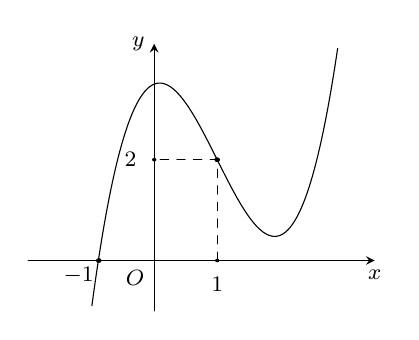
\begin{tikzpicture}[scale=0.8,>=stealth, font=\footnotesize, line join=round, line cap=round,yscale=0.8]
	\def\a{1} \def\b{-3} \def\c{0.5} \def\d{3.5} % Hệ số
	\def\xmin{-2} \def\xmax{3.5}
	\def\ymin{-1} \def\ymax{4.3} 
	\draw[->] (\xmin,0)--(\xmax,0) node [below]{$x$};
	\draw[->] (0,\ymin)--(0,\ymax) node [left]{$y$};
	\node at (0,0) [below left]{$O$};
	\clip (\xmin+0.1,\ymin+0.1) rectangle (\xmax-0.5,\ymax-0.1);
	\draw[smooth,samples=300] plot(\x,{\a*(\x)^3+\b*(\x)^2+\c*(\x)+\d});
	\node at (-1.2,-0.3){$-1$};
	\draw[fill=black] (-0.88,0) circle(1pt) (1,2) circle(1pt);
	\draw[dashed] (1,0)|-(0,2);
	\foreach \s/\t in {1/-90}
	\fill (\s,0) circle (1pt) node[shift={(\t:3mm)}]{$\s$};
	\foreach \p/\r in {2/180}
	\fill (0,\p) circle (1pt) node[shift={(\r:3mm)}]{$\p$};
\end{tikzpicture}
}
\loigiai{
\immini{ 
	Ta có 
	\begin{eqnarray*}
	g'(x) &= &\cos x \cdot f' (\sin x -1) - \dfrac{1}{2} \sin 2x = \cos x \left[ f'(\sin x -1) -\sin x \right]\\
	& = & \cos x \left[ f'(\sin x -1) -(\sin x-1+1 ) \right] 
	\end{eqnarray*}
Vẽ thêm đường thẳng $y=x+1$.\\ Ta có $f'(x) - (x+1)$ cùng dấu với $(x+1)(x-1)(x-a)$, $(a>1)$.
}{
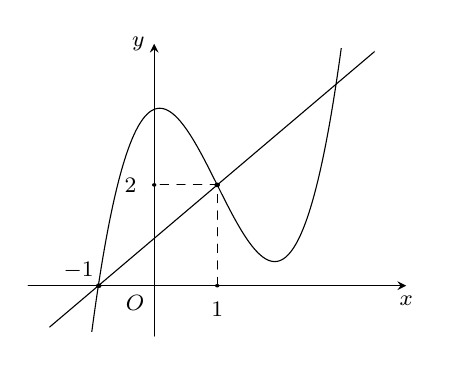
\begin{tikzpicture}[scale=0.8,>=stealth, font=\footnotesize, line join=round, line cap=round,yscale=0.8]
	\def\a{1} \def\b{-3} \def\c{0.5} \def\d{3.5} % Hệ số
	\def\xmin{-2} \def\xmax{4.0}
	\def\ymin{-1} \def\ymax{4.8} 
	\draw[->] (\xmin,0)--(\xmax,0) node [below]{$x$};
	\draw[->] (0,\ymin)--(0,\ymax) node [left]{$y$};
	\node at (0,0) [below left]{$O$};
	\clip (\xmin+0.1,\ymin+0.1) rectangle (\xmax-0.5,\ymax-0.1);
	\draw[smooth,samples=300] plot(\x,{\a*(\x)^3+\b*(\x)^2+\c*(\x)+\d});
	\node at (-1.2,0.3){$-1$};
	\draw[fill=black] (-0.88,0) circle(1pt) (1,2) circle(1pt);
	\draw[dashed] (1,0)|-(0,2);
	\foreach \s/\t in {1/-90}
	\fill (\s,0) circle (1pt) node[shift={(\t:3mm)}]{$\s$};
	\foreach \p/\r in {2/180}
	\fill (0,\p) circle (1pt) node[shift={(\r:3mm)}]{$\p$};
	\draw (-1.66,-0.82)--(3.7,4.86);
\end{tikzpicture}
}
 \noindent Nên g'(x) cùng dấu với $\cos x ( \sin x -1 +1)(\sin x -1 -1)(\sin x -1 -a) = \cos x \sin x (\sin x -2) [ \sin x -(1+a)]$ cùng dấu với $\cos x \sin x =\dfrac{1}{2} \sin 2x$ ( do $(\sin x -2) [ \sin x -(1+a)] >0$).\\
 Ta lại có $\sin 2x $ đổi dấu từ âm sang dương $5$ lần trên khoảng $\left( -\dfrac{\pi}{2};5\pi \right)$ nên hàm số $g(x)$ có $5$ điểm cực tiểu.
 \begin{center}
 	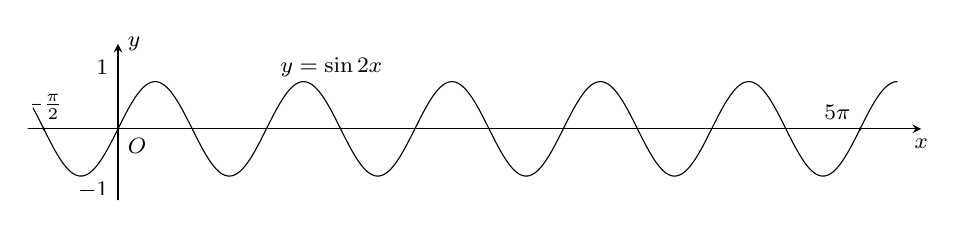
\begin{tikzpicture}[scale=0.6,>=stealth, font=\footnotesize, line join=round, line cap=round]
 	\def\xmin{-1.9} \def\xmax{17} \def\ymin{-1.5} \def\ymax{1.8}
 	\draw[->] (\xmin,0)--(\xmax,0) node [below]{$x$};
 	\draw[->] (0,\ymin)--(0,\ymax) node [right]{$y$};
 	\node at (0,0) [below right]{$O$};
 	\clip (\xmin+0.1,\ymin+0.1) rectangle (\xmax-0.5,\ymax-0.1);
 	\draw[smooth,samples=400,domain=\xmin:\xmax] plot(\x,{sin(2*\x r)});
% 	\draw[dashed] (\xmin,1)--(\xmax,1) (\xmin,-1)--(\xmax,-1);
 	\node at (0,1.3) [left]{$1$};
 	\node at (0,-1.3) [left]{$-1$};
 	\node at (-0.5*pi,0) [above]{$-\frac{\pi}{2}$};
 	\node at (5*pi,0) [above left]{$5\pi$};
	\foreach \s in {-0.5*pi,5*pi}
	\fill (\s,0) circle (1pt);
	\node at (5.8,1.3) [left]{$y=\sin 2x$};
 	\end{tikzpicture}
 \end{center}
}
\end{ex}
%%==========Câu 49
\begin{ex}%[Dự án 12-Vted-2022, Phan Quốc Trí]%[2D2G6-5]
Có bao nhiêu số nguyên $y \in [-30; 30]$ sao cho ứng với mỗi $y$ tồn tại ít nhất $12$ số nguyên $x$ thỏa mãn 
$$\left(9x^2 + 9 \right) \left(3^{2xy-y} -3^{x^2-1}\right) \ge \dfrac{x^2-2xy+y-1}{2xy-y+2}?$$ 
\choice
{\True $49$}
{$10$}
{$51$}
{$12$}
\loigiai{
$$\left(9x^2 + 9 \right) \left(3^{2xy-y} -3^{x^2-1}\right) \ge \dfrac{x^2-2xy+y-1}{2xy-y+2} \Leftrightarrow 3^{2xy-y+2} -3^{x^2+1} \ge \dfrac{x^2-2xy+y-1}{(x^2+1)(2xy-y+2)}. $$
Đặt $a=2xy -y +2$; $b = x^2 +1$, ($b \ge 1$) $\Rightarrow 3^{a} - 3^{b} \ge \dfrac{b-a}{ab}=\dfrac{1}{a} - \dfrac{1}{b} \Leftrightarrow 3^{a} - \dfrac{1}{a} \ge 3^{b} - \dfrac{1}{b} \quad (*)$\\
Hàm số $g(t) = 3^{t} - \dfrac{1}{t} $ có $g'(t) = 3^{t} \ln 3 + \dfrac{1}{t^2}> 0$, $ \forall t \ne 0 $ nên đồng biến trên mỗi khoảng $(- \infty; 0)$; $(0;+\infty)$.
\begin{itemize}
	\item [\bf TH1.] Nếu $a>0 \Rightarrow a,b \in (0;+ \infty)$. Khi đó $(*) \Leftrightarrow g(a) \ge g(b) \Leftrightarrow a \ge b$.
	\item [\bf TH2.] Nếu $a<0$ khi đó giả sử tồn tại các số ngyên $x$, $y$ thỏa mãn đề bài khi đó ta cũng có $a$, $b \in \mathbb{Z} \Rightarrow a \le -1; b \ge 1 \Rightarrow g(a) \le g(-1) = \dfrac{4}{3}$; $g(b) \ge g(1) = 2$ nên sẽ không thỏa mãn $(*)$. 
\end{itemize}
Vậy tóm lại điều kiện là $a\ge a \Leftrightarrow 2xy -y +2 \ge x^2 +1 \Leftrightarrow (x-y)^2 \le y^2 -y +1 \Leftrightarrow x-y \in \left[-\sqrt{y^2-y+1};\sqrt{y^2-y+1} \right]$ chứa ít nhất $12$ số nguyên $x \Leftrightarrow $ chứa ít nhất $12$ số nguyên $x-y$ là các số $-6, \ldots , 6 \Leftrightarrow \sqrt{y^2-y+1} \ge 6 \Rightarrow y \in \left\{-30, \ldots,-6,7,\ldots 30 \right\}$. 
}
\end{ex}
%%==========Câu 50
\begin{ex}%[Dự án 12-Vted-2022, Phan Quốc Trí]%[2D4G5-1]
Xét hai số phức $z_1$, $z_2$ thỏa mãn $\left| z_1+2 \right| +\left| z_1-1 \right| +\left| z_1- \overline{z_1} -2 \right| =5 $ và $ \left| i \cdot z_2 +3 - 2i \right| = 2$. Khi $\left| z_1 - z_2 \right| $ đạt giá trị lớn nhất thì $\left| i \cdot z_1 + z_2 -1 \right| $ bằng
\choice
{$\dfrac{\sqrt{65}}{5}$}
{$\dfrac{\sqrt{185}}{5}$}
{\True $\dfrac{\sqrt{290}}{5}$}
{$\dfrac{8\sqrt{5}}{5}$}
\loigiai{
Đặt $z_1=x+yi \; (x,y \in \mathbb{R})$. Gọi $M$, $N$ lần lượt là điểm biểu diễn của các số phức $z_1$, $z_2$. Ta có 
$$\left| z_1 +2 \right| + \left| z_1 -1 \right| +\left| z_1 - \overline{z_1} -2 \right| = 5 \Leftrightarrow \sqrt{(x-2)^2 + y^2} + \sqrt{(x-1)^2 + y^2} + \sqrt{4y^2+4}= 5. \quad(*) $$
Mặt khác 
$$VT_{(*)} \ge \sqrt{(x+2)^2} + \sqrt{(x-1)^2} + \sqrt{4} = \left| x+2 \right| + \left| 1-x \right| +2 \ge \left| (x+2) + (1-x) \right| +2 = 5 = VP_{(*)}.$$
Dấu bằng xảy ra khi $\heva{&y=0 \\& (x+2)(1-x) \ge 0} \Leftrightarrow \heva{&y=0 \\& -2 \le x \le 1 }$. Vậy $M$ thuộc đoạn $AB$ với $A(-2;0)$, $B(1;0)$.\\
Và $\left| i \cdot z_2 + 3-2i \right| = 2 \Leftrightarrow \left| i \left(z_2 + \dfrac{3}{i} -2\right) \right| = 2 \Leftrightarrow \left| z_2 -2 -3i \right| = 2$.
\immini{
Vậy $N$ thuộc đường tròn tâm $I(2;3)$, bán kính $R=2$. \\
Khi đó $\left| z_1 - z_2 \right| = MN \le IM + IN = IM + R \le \max \left\{IA,IB\right\} +R = \max \left\{5,\sqrt{10}\right\} +2 = 5+2=7$.\\
Dấu bằng xảy ra khi $M$ trùng $A(-2;0)$. Suy ra $z_1=-2$ và $A$, $I$, $N$ thẳng hàng theo thứ tự. Do đó 
$$\overrightarrow{IN} = \dfrac{IN}{AI} \overrightarrow{AI} = \dfrac{2}{5} (4;3) \Rightarrow N \left(\dfrac{18}{5}; \dfrac{21}{5}\right) \Rightarrow z_2 =\dfrac{18}{5} + \dfrac{21}{5}i .$$
}{
	\begin{tikzpicture}[scale=0.7,>=stealth, font=\footnotesize, line join=round, line cap=round]
	\draw[->] (-3,0)--(6,0) node [below]{$x$};
	\draw[->] (0,-1)--(0,5) node [left]{$y$};
%	\clip (-6,-6) rectangle (6,6);
	\coordinate (I) at (2,3);
	\coordinate (A) at (-2,0);
	\coordinate (M) at (-0.8,0);
	\coordinate (B) at (1,0);
	\draw (I) circle(2cm);
	\coordinate (N) at ($(I)+(320:2cm and 2cm)$);
	\draw[dashed] (2,0)|-(0,3);
	\foreach \p/\r in {I/90, A/90, M/-90, B/140, N/-20}
	\fill (\p) circle (1pt) node[shift={(\r:3mm)}]{$\p$};
	\foreach \s/\t in {-2/-90,1/-90,2/-90}
	\fill (\s,0) circle (1pt) node[shift={(\t:3mm)}]{$\s$};
	\foreach \p/\r in {3/180 }
	\fill (0,\p) circle (1pt) node[shift={(\r:3mm)}]{$\p$};
	\draw (N)--(I)--(A) (B)--(I)--(M)--(N);
\end{tikzpicture}
}
Khi đó $\left| i \cdot z_1 + z_2 -1 \right| = \left| -2i +\dfrac{18}{5} + \dfrac{21}{5}i -1 \right| = \dfrac{\sqrt{290}}{5}$.
}
\end{ex}
\Closesolutionfile{ans}
\inputansbox{10}{ans/ans-Vted-19-2023}